\begin{frame}
    \frametitle{Konsequenzen der Riemannschen Hypothese}
    \only<1>{
        \begin{lemma}
            \[
                \sigma(n) = \sum_{d | n} d < e^\gamma n \log \log n + \frac{0.6483\ n}{\log \log n}
            \]
        \end{lemma}
        \begin{theorem}[Robin, 1984]
            Die Abschätzung \[
                \sigma(n) < e^\gamma n \log \log n 
                    \]
            ist äquivalent zur Riemannschen Hypothese.
        \end{theorem}
    }
    \only<2>{
        \begin{figure}
            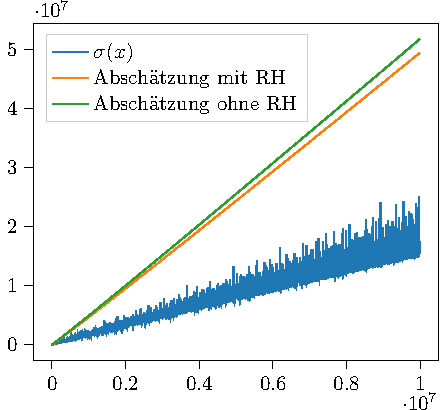
\includegraphics[scale=0.9]{figures/robins_inequality_plot.pdf}
        \end{figure}
    }
\end{frame}